\documentclass[main.tex]{subfiles}
Resources for this section are my own lecture notes from Professor Corwin's Fall 2019 Analysis \& Probability I course and \textit{Probability Theory and Examples, 5th ed.} By Rick Durrett.

\subsection{Basic Measure Theory}
\subsubsection{Definition of a Measure and Basic Properties}
\begin{definition}[$\sigma$-algebra]
Let $\om$ be a set. We say $\cF \subset 2^{\om}$ is a $\sigma$-algebra if,
\begin{enumerate}
    \item $\om \in \cF$
    \item If $A \in \cF$, then $A^c \in \cF$ as well
    \item For every countable collection $\{A_i\} \subset \cF$, $\bigcup A_i \subset \cF$ as well
\end{enumerate}
Note that given 2 we could equivalently require that 1 read $\phi \in \cF$ and that 3 read that $\cF$ is closed to countable intersections.
\end{definition}

\begin{definition}[Measurable Space]
A pair $(\om, \cF)$ is called a measurable space.
\end{definition}

\begin{definition}[Measure and Probability Measure]
A measure $\mu$ on $(\om, \cF)$ is any countably additive, non-negative function, $\mu: \cF \to \R_{\geq 0}$ i.e. 
\begin{enumerate}
    \item $\mu(A) \geq \mu(\phi) = 0$
    \item $\mu(\bigcup_i A_i) \leq \sum_i \mu(A_i)$ with equality holding if the $A_i$ are disjoint (or if their intersections have measure 0)
\end{enumerate}
If $\mu(\om) = 1$, then we call $\mu$ a probability measure and often denote it by $\prob$.
\end{definition}

\begin{definition}
A measure $\mu$ on $(\om, \cF)$ is $\sigma$-finite if $\om = \bigcup_i A_i$ for $A_i \in \cF$ and $\mu(A_i) < \infty$ for all $i$.
\end{definition}
\begin{example}
All finite measures are $\sigma$-finite.
\end{example}
\begin{example}
The Lebesgue measure on $\R$ is $\sigma-finite$ with $A_i = [i, i+1]$ for $i \in \mathbb{Z}$
\end{example}

\begin{definition}[Measure Space and Probability Space]
We say that a triple $(\om, \cF, \mu)$ is a measure space. If $\mu$ is a probability measure, we call it a probability space.
\end{definition}

\begin{prop}
Given a probability space $(\om, \cF, \prob)$, the following hold,
\begin{enumerate}
    \item Monotonicity: if $A \subset B$, then $\prob(A) \leq \prob(B)$
    \item Continuity from above: if $A_1 \subset A_2 \subset ...$ such that $\bigcup_i A_i = A$ then $\prob(A_i) \to \prob (A)$
    \item Continuity from below: if $A_1 \supset A_2 \supset ...$ and $\bigcap_i A_i = A$ then $\prob(A_i) \to \prob(A)$
\end{enumerate}
\end{prop}

The proof of these properties follows pretty immediately from the definition.

\begin{prop}
For any collection $\cF \subset 2^{\om}$, there exists a unique $\sigma$-algebra $\sigma(\cF)$ such that,
\begin{enumerate}
    \item $\cF \subset \sigma(\cF)$
    \item for all $\sigma$-algebras $\mathcal{B}$ such that $\cF \subset \mathcal{B}$, $\sigma(\cF) \subset \mathcal{B}$
\end{enumerate}
\end{prop}
\begin{remark}
This construction requires the axiom of choice \textcolor{red}{why?}.
\end{remark}


\subsubsection{Carathéodory Extension Theorem}

We can use these minimally generated $\sigma$-algebras to define measures on spaces. First, we say that $\mathcal{A} \subset 2^{\om}$ is an algebra if it contains $\om$ and is closed to compliments and finite unions. 

\begin{theorem}[Carathéodory Extension Theorem]
Given a function,
\[\mu_0: \mathcal{A} \to \R_{\geq 0}\]
that is countably additive (known as a premeasure), there exists a measure,
\[\mu: \sigma(\mathcal{A}) \to \R_{\geq 0}\]
extending $\mu_0$, and if $\mu_0(\om) < \infty$ (known as being finite), then $\mu$ is unique.
\end{theorem}

\begin{proof}
We begin by defining an outer measure,$\mu^*: 2^{\om} \to \R \cup \{+\infty\}$ via the following formula:
\[\mu^*(A) = \inf\{\sum_i \mu (A_i)| A_i \in \cA, \bigcup_i A_i \supset A\}\]
Note that we can assume that the $A_i$ are disjoint by the countably additive assumption on $\mu$. We prove the following properties of this outer measure:
\begin{enumerate}
    \item Monotonicity
    \item Countably Subadditive
    \item $\mu^* = \mu$ on $\cA$
\end{enumerate}
Monotonicity is clear from the definition. For countably subadditve, we need to show,
$$\mu^*(\bigcup_i A_i) \leq \sum_i \mu^*(A_i)$$
Fix $\vep > 0$. There exists a $B_{i,j} \in \cA$ such that $\bigcup_j B_{i,j} \supset A_i$ and $\sum_j \mu(B_{i,j})\leq \mu^*(A_i) + \vep/2^i$ by definition of infimum. Then we have that,
\[\sum_i \mu^*(A_i) + \vep \geq \sum_{i,j} \mu(B_{i,j}) \geq \mu(\bigcup_{i,j}B_{i,j}) \geq \mu^*(\bigcup_i A_i)\]
where the second inequality follows from countable additivity on $\cA$ and the last follows by monotonicity.

To see that $\mu^* = \mu$ on $\cA$, note that by the countably additive property of $\mu$ the quantity $\sum_i \mu(A_i)$ for $A \subset \bigcup_i A_i$ is minimized when $A = \bigcup_i A_i$ and $\sum_i \mu(A_i) = \mu(\bigcup_i A_i) = \mu(A).$

We now define a subset $E \subset \om$ to be \textit{measurable} if for all other $A \subset \om$,
\[\mu^*(A) = \mu^*(A \cap E) + \mu^*(A \cap E^c)\]
Note that by the properties we've proven $\leq$ follows immediately, so we really only need to check $\geq$. We define $\cM$ to be the collection of all measurable sets. First we show that $\cM$ is an algebra.

\textcolor{red}{FINISH}

\end{proof}

The standard $\sigma$-algebra on $\R$ is the Borel $\sigma$-algebra $\cB$ defined as $\sigma(\mathcal{A})$ for $\mathcal{A} = \{(a_1,b_1] \cup .... \cup (a_k, b_k] | a_1 < b_1 < ... < a_k < b_k\}$. We define measures on $(\R, \cB)$ via distribution functions:

\begin{definition}
A Lebesgue-Steiljes distribution function $F: \R \to \R$ is a function that is non-decreasing and right continuous. Additionally, if $F(-\inf) = 0$ and $F(+\inf) = 1$, we call it a probability distribution function.
\end{definition}

We use these distribution functions to define measures on $\R$ by defining them on the generating algebra $\cA$ of $\cB$ to be,
\[\mu(\bigcup_{i = 1}^k (a_i, b_i]) = \sum_{i = 1}^{k} (F(b_i) - F(a_i))\]
In probability language, $F$ is the \textit{Cumulative Distribution Function} or CDF. When $F(x) = x$, we call the resulting measure the \textit{Lebesgue Measure} on $\R.$

\textcolor{red}{Include some comments about the space of measurable sets $\cM$ and how we define them via the axiom of choice}

\subsubsection{Measurable Functions and Random Variables}
We now move on to discussing the morphisms in the category of measurable spaces, measurable functions.
\begin{definition}[Measurable Function]
A function $X: (\om, \cF) \to (\om', \cF')$ is \textit{measurable} if for every $E \in \cF'$, $X^{-1}(E) \in \cF.$
\end{definition}

\begin{definition}[Random Variable and Random Vector]
If $(\om, \cF, \prob)$ is a probability space, and $X:(\om, \cF) \to (\R^d, \cB)$ is measurable, then $X$ is a random vector. In the case $d = 1$, $X$ is a random variable
\end{definition}


\begin{theorem}
If $\cA$ is a collection of subsets in $\om'$ such that $\sigma(\cA) = \cF'$, then $X$ is measurable if and only if for all $E \in \cA$, $X^{-1}(E) \in \cB$. That is, it is sufficient to check measurability on a generating set of your $\sigma$-algebra.
\end{theorem}
\begin{proof}
\textcolor{red}{Proof needed}
\end{proof}


\begin{definition}
For a function $X: (\om, \cF) \to (\om', \cF'),$ define $\sigma(X)$ to be the smallest $\sigma$-algebra on $\om$ such that $X: (\om, \sigma(X)) \to (\om', \cF')$ is measurable.
\end{definition}
\begin{remark}
Note that this construction also depends on $\cF$.
\end{remark}

\begin{prop}
A function $Y:(\om, \sigma(X)) \to (\om'', \cF'')$ is measurable if and only if $Y = f \circ X$ for some $f: (\om', \cF') \to (\om'', \cF'')$ measurable.
\end{prop}
\begin{proof}
\textcolor{red}{Proof needed QUESTION: IS THIS ONLY TRUE IN BOREL? Possible counter example: $\cF$ is the trivial $\sigma$-algebra}
\end{proof}

\begin{prop}
If $X, Y$ are measurable functions $(\om, \cF) \to (\R, \cB)$, then so are $X + Y$, $cX, XY,$ $\max(X,Y),$ $\min(X,Y),$ $\inf_n X_n,$ $sup_n X_n,$ $\liminf_x X_n,$ $\limsup_n X_n$. For $\{X_n\}_{n \geq 0}$, the set $\om = \{\omega \in \om| \lim(X_i(\omega)) \text{ exists}\}$ is a measurable set. \textcolor{red}{meaning it is in $\cF$?}
\end{prop}


\begin{theorem}[Lusin's]
If $f: \R \to \R$ is Borel measurable, then for all $\vep > 0$ there exists a continuous $g: \R \to \R$ such that the set $\{x|f(x) = g(x)\}$ is closed and the compliment has Lebesgue measure $\leq \vep$
\end{theorem}
\textcolor{red}{Check the statement of this because it was wonky in my notes}
In other words, any measurable function $f: \R \to \R$ can be closely approximated by a continuous function $g$. 

Now we consider how a measurable map pushes forward a measure on $(\om, \cF)$ to a measure on $(\om', \cF')$.

\begin{definition}[Distribution Function]
Let $(\om, \cF, \prob)$ be a probability space, $X$ a random variable. The distribution function of $X$, $F_X: \R \to [0,1]$ is defined by,
\[F_X(x) = \prob(\{\omega \in \om| X(\omega) \leq x
\})\]
Furthermore, this function defines a probability measure on $(\R, \cB)$.
\end{definition}
\begin{remark}
Random variables are \textit{not} defined by their distribution functions.
\end{remark}

\begin{prop}
All distribution functions have the following properties:
\begin{enumerate}
    \item Non-decreasing
    \item $\lim_{x \to +\infty} F(X) = 1, \lim_{x \to -\infty} F(X) = 0$
    \item Right continuous
    \item Left limits exist and are equal to $\prob(X < x)$ (we denote these limits as $F(x-)$)
    \item $F(x) - F(x-) = \prob(X = x)$
\end{enumerate}
\end{prop}

\subsubsection{Integration}
The goal of this section is to define integration with respect to a $\sigma$-finite measure $\mu$ on a measurable space $(\om, \cF)$. We construct $\int_{\om} f d\mu$ in 4 steps, at each stage we can verify the following properties:
\begin{enumerate}
    \item If $\varphi \geq 0$ almost everywhere, then $\int \varphi d\mu \geq 0$
    \item For all $a \in \R$, $\int a \varphi d\mu = a \int \varphi d \mu$. 
    \item $\int (\varphi + \psi) d\mu = \int \varphi d \mu + \int \psi d \mu$
    \item If $\varphi \leq \psi$ almost everywhere, $\int \varphi d \mu \leq \int \psi d \mu$
    \item $|\int \varphi d \mu| \leq \int |\varphi| d \mu$
\end{enumerate}

\paragraph{Step 1} For $\varphi$ a simple function $\varphi = \sum_{i = 1}^n a_i 1_{A_i}$, with $A_i$ disjoint measurable sets with $\mu(A_i) < \infty$, we define,
\[\int \varphi d \mu = \sum_{i = 1}^n a_i \mu(A_i)\]

\paragraph{Step 2} For $f$ bounded and $f = 0$ outside some $E$ such that $\mu(E) < \infty$, we define,
\[\int f d\mu = \sup_{\varphi \leq f} \int \varphi d \mu = \inf_{\psi \geq f} \int \psi d \mu\]
To prove that this equality is true, we can approximate our function $f$ from above and below by simple functions via the following sequences:
\[\psi_n = \sum_{k = -n}^n \frac{kM}{n}1_{f^{-1}([\frac{(k-1)M}{n}, \frac{kM}{n}])} \quad \quad \varphi_n = \sum_{k = -n}^n \frac{(k-1)M}{n}1_{f^{-1}([\frac{(k-1)M}{n}, \frac{kM}{n}])}\]
\begin{remark}
Note that, as opposed to Riemannian integration, this allows us to subdivide based on our range instead of our domain. This allows us to integrate more functions, for instance,
\[f(x) = \begin{cases}
1 & x \in \mathbb{Q}\\
0 & \text{else}
\end{cases}\]
can now be integrated on any bounded subset of $\R$.
\end{remark}

\paragraph{Step 3} For $f \geq 0$, we define,
\[\int f d\mu = \sup \{\int h d \mu| 0 \leq h \leq f, ||h||_{\infty} < \infty, \mu(\{x | h(x) \neq 0)\})<\infty\}\]

\paragraph{Step 4} Let $f$ be such that, as defined above, $\int|f| d \mu < \infty$ (we say $f$ is \textit{integrable}). Define,
\[f^-(x) = \begin{cases}
-f(x) & f(x) \leq 0\\
0 & \text{else}
\end{cases}
\quad \quad f^+(x) = \begin{cases}
f(x) & f(x) \geq 0\\
0 & \text{else}
\end{cases}\]
Then we define,
\[\int f d\mu = \int f^+ d\mu - \int f^- d\mu\]
\begin{remark}
For intuition as to why this is the correct notion of ``integrable", note that in the countable case we want to define the integral to be $\sum_{i \in \om} f(i) \mu(i)$, however if we do not have that this sum converges absolutely, that is, if $\sum_{i \in \om} |f(i)|\mu(i) = \infty$, then the sum $\sum_{i \in \om} f(i) \mu(i)$ can be rearranged to equal whatever value we want. This is clearly not a well defined notion of integration.
\end{remark}

The following is common notation for specific types of integrals,
\begin{enumerate}
    \item $(\R^d, \cB, \text{Lebesgue})$: $\int_A f(x) dx$
    \item $\om$ countable: $\int f d\mu = \sum_{i \in \om} f(i) \mu(i)$
    \item $(\R, \cB, \mu)$ with $\mu([a,b]) = G(b) - G(a)$: $\int f d\mu = \int f(x) dG$
\end{enumerate}

\begin{definition}[Expectation]
Let $\prob$ be a probability measure and $X$ a positive random variable. Then we define $\E[X] = \in X d\prob$. If $X$ is not necessarily $\geq 0$, we define $\E[X] = \int x^+ d\prob - \int X^- d\prob$ provided both $X^+$ and $X^-$ are integrable. A random variable $X$ is integrable if $\E[X] < \infty.$
\end{definition}

Now we can prove the first of the Borel-Cantelli lemmas:

\begin{definition}
    For $\{A_n\}_n$ a sequence of subsets in $\om$, 
    \[\limsup_{n \to \infty} A_n = \lim_{m \to \infty} \bigcup_{n = m}^{\infty} A_n = \limsup_{n \to \infty} 1_{A_n}\]
    (i.e. the set of all $\omega \in \om$ such that $\omega \in A_k$ for infinite $k$)
    \[\liminf_{n \to \infty} A_n = \lim_{m \to \infty} \bigcap_{n = m}^{\infty} A_n = \liminf_{n \to \infty} 1_{A_n}\]
    (i.e. the set of all elements $\omega \in \om$ such that $\omega \in A_k$ for all but finitely many $k$.
\end{definition}
    
\begin{lemma}[Borel-Cantelli Lemma (1)]
    If $\sum_{n = 1}^{\infty} \prob(A_n) < \infty$, then $\prob(\limsup_{n \to \infty} A_n) = 0$
\end{lemma}
    \begin{proof}
    Let $N(\omega) = \sum_{k = 1}^{\infty} 1_{A_k}(\omega)$. Then $\E[|N|] = \E[N] = \sum_{k = 1}^{\infty} \prob(A_k) < \infty$, therefore $N$ must be $< \infty$ almost surely.
\end{proof}
\begin{remark}
    The converse to this (that if the probabilities of the sets are not summable the $\limsup$ occurs with positive probability) is not true.
\end{remark}




\begin{prop}[Jensen's Inequality]
For $\varphi: \R \to \R$ convex, 
\[\varphi(\int f d \mu) \leq \int \varphi(f) d \mu\]
\end{prop}


\begin{prop}[Holder's Inequality]
For $p,q \in (1,\infty)$ such that $\frac{1}{p} + \frac{1}{q} = 1$,
\[\int |fg| d \mu = ||fg||_1 \leq ||f||_p||g||_q\]
where $||f||_p = (\int |f|^pd\mu)^{1/p}$
\end{prop}
\begin{remark}
When $p = q = 2$, this is Cauchy-Schwartz inquality.
\end{remark}

\begin{prop}[Markov Inequality]
    \textcolor{red}{Need statement and proofs for all of the above ALSO CHEBYSHEV!}
\end{prop}


\begin{definition}[Product Measure]
Let $(X, \cA, \mu_1), (Y, \cB, \mu_2)$ be $\sigma$-finite measure spaces. Let $\om = X \times Y$, $S = \{A \times B| A \in \cA, B\in \cB\}, \sigma(S) = \cF$. Then the product measure $\mu = \mu_1 \times \mu_2$ on $(\om, \cF)$ is defined to be the Cáratheodory extension of the measure defined on $S$ by $\mu(A \times B) = \mu_1(A)\mu_2(B)$. 
\end{definition}
\begin{remark}
Visually, we can think of this measure in $\R^2$ as being defined on rectangles by length $\times$ width and defined on other sets as the limit of approximating the set by a covering of smaller and smaller rectangles and taking their measures.
\end{remark}

\begin{theorem}[Fubini's Theorem]
If $f \geq 0$ or $\int|f| d \mu < \infty$, then,
\[\int_{X \times Y} f d\mu = \int_X \int_Y f(x,y) \mu_2(dy) \mu_1(dx)\]
\end{theorem}
\begin{proof}
\textcolor{red}{Proof Needed (in Durrett, not in my notes)}
\end{proof}





\subsection{Convergence}
\subsubsection{Convergence Theorems for Integrals}

\begin{definition}[Convergence in Measure]
A sequence of functions $f_n: \om \to \R$ converges in measure to $f: \om \to \R$ if for all $\varepsilon > 0$,
\[\lim_{n \to \infty} \mu(|f_n - f| > \vep) = 0\]
\end{definition}

\begin{theorem}[Bounded Convergence Theorem]
    Assume there exists some $E \subset \om$ such that $\mu(E) > 0$ and there exists some $M> 0$ such that for all $n$, $f_n = 0$ on $E^c$ and $||f_n||_{\infty} < M$, and assume that $f_n \to f$ in measure. Then,
    \[\lim_{n \to \infty} \int f_n d\mu = \int f d\mu\]
\end{theorem}
\begin{proof}
    \textcolor{red}{Proof needed}
\end{proof}

\begin{theorem}[Fatou's Inequality]
    If $f_n \geq 0$, then 
    \[\liminf_{n \to \infty} (\int f_n d\mu) \geq \int (\liminf_{n \to \infty} f_n)d\mu \]
\end{theorem}
\begin{proof}
    \textcolor{red}{Proof needed}
\end{proof}

\begin{theorem}[Monotone Convergence Theorem]
    If $f_n \geq 0$ and $f_n \nearrow f$ monotonically, then $\int f_n d\mu \nearrow \int fd\mu$
\end{theorem}
\begin{proof}
    \textcolor{red}{Proof needed}
\end{proof}

\begin{theorem}[Dominated Convergence Theorem]
    If $f_n \xrightarrow{a.e.} f$, and $|f_n| \leq g$ for $g$ integrable, then $\lim_{n \to \infty} f_n d \mu \to \int f d\mu$
\end{theorem}
\begin{proof}
    \textcolor{red}{Proof needed}
\end{proof}

\subsubsection{Convergence of Random Variables}

\begin{definition}[Almost Sure Convergence]
    A sequence of random variables $\{X_n\}_n$ converges almost surely to $X$ (denoted $X_n \xrightarrow{a.s.}X$) if $\prob(\{\omega \in \om| X_n(\omega) \text{ does not converge to }X(\omega)\}) = 0$
\end{definition}

\begin{definition}[Convergence in Probability]
    A sequence of random variables $\{X_n\}_n$ defined on the same probability space converges in probability to a random variable $X$ (denoted $X_n \xrightarrow{p} X$) if they converge in measure with respect to $\prob$.
\end{definition}
    \begin{remark}
    This definition is weaker than almost sure convergence. For example, consider the following sequence of random variables on $[0,1]$ with uniform measure: For each $k \in \mathbb{N}$ we subdivide $[0,1]$ into $k$ segments of length $\frac{1}{k}$ and label the $i$-th segment of length $\frac{1}{k}$ $k_i$. Then we get the following sequence of segments $1_1, 2_1, 2_2, 3_1, 3_2, 3_3, 4_1,...$. Define $X_n$ to be 1 on the $n$-th segment in this sequence and 0 otherwise. Then we have that for any $0 < \vep < 1$, if $X_n = k_i, \prob(|X_n - X|> \vep) = \frac{1}{k} \to 0$, however for every $x \in [0,1]$ the sequence $X_n(x)$ does not converge, so this sequence does not converge almost surely (or even anywhere). The first few instances elements of this sequence are illustrated below:
    \begin{center}
    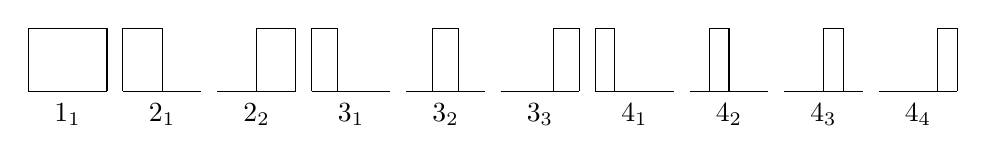
\begin{tikzpicture}
    \draw (-2.3, 0) -- (-1.3, 0); %bottom line
    \draw (-2.3, .8) -- (-1.3, .8); %top line
    \draw (-1.3, .8) -- (-1.3, 0); \draw (-2.3, .8) -- (-2.3, 0); %legs
    \draw (-1.8,-.3) node {$1_1$};

    \draw (-1.1,.8) -- (-.6,.8); \draw (.6, .8) -- (1.1, .8);
    \draw (-1.1, .8) -- (-1.1, 0); \draw(-.6,.8) -- (-.6, 0); \draw (.6, .8) -- (.6, 0); \draw (1.1, .8) -- (1.1, 0);
    \draw (-1.1,0) -- (-.1,0); \draw(.1, 0) -- (1.1,0);
    \draw (-.6,-.3) node {$2_1$};
    \draw (.6,-.3) node {$2_2$};

    \draw (1.3, 0) -- (2.3, 0); %bottom line
    \draw (1.3, .8) -- (1.63, .8); %top line
    \draw (1.3, .8) -- (1.3, 0); \draw (1.63, .8) -- (1.63, 0); %legs
    \draw (1.8,-.3) node {$3_1$};

    \draw (2.5, 0) -- (3.5, 0); %bottom line
    \draw (2.83, .8) -- (3.16, .8); %top line
    \draw (3.16, .8) -- (3.16, 0); \draw (2.83, .8) -- (2.83, 0); %legs
    \draw (3,-.3) node {$3_2$};

    \draw (3.7, 0) -- (4.7, 0); %bottom line
    \draw (4.37, .8) -- (4.7, .8); %top line
    \draw (4.37, .8) -- (4.37, 0); \draw (4.7, .8) -- (4.7, 0); %legs
    \draw (4.2,-.3) node {$3_3$};

    \draw (4.9, 0) -- (5.9, 0); %bottom line
    \draw (4.9, .8) -- (5.15, .8); %top line
    \draw (4.9, .8) -- (4.9, 0); \draw (5.15, .8) -- (5.15, 0); %legs
    \draw (5.4,-.3) node {$4_1$};

    \draw (6.1, 0) -- (7.1, 0); %bottom line
    \draw (6.35, .8) -- (6.6, .8); %top line
    \draw (6.6, .8) -- (6.6, 0); \draw (6.35, .8) -- (6.35, 0); %legs
    \draw (6.6,-.3) node {$4_2$};

    \draw (7.3, 0) -- (8.3, 0); %bottom line
    \draw (7.8, .8) -- (8.05, .8); %top line
    \draw (7.8, .8) -- (7.8, 0); \draw (8.05, .8) -- (8.05, 0); %legs
    \draw (7.8,-.3) node {$4_3$};

    \draw (8.5, 0) -- (9.5, 0); %bottom line
    \draw (9.25, .8) -- (9.5, .8); %top line
    \draw (9.25, .8) -- (9.25, 0); \draw (9.5, .8) -- (9.5, 0); %legs
    \draw (9,-.3) node {$4_4$};
    \end{tikzpicture}
    \end{center}
\end{remark}


\begin{prop}
    A sequence of random variables $\{X_n\}_n$ converges in probability to $X$ if and only if for every subsequence $n(k)$ there exists a further subsequence $\{X_{n(k_j)}\}_j$ that converges almost surely to $X$.
\end{prop}
\begin{proof}
    To prove convergence in probability implies every subsequence has a almost surely convergent further subsequence it is sufficent to check this just for the entire sequence (since any subsequence converges in probability as well).This direction of the proposition is an application of the first Borel-Cantelli Lemma. For all $k \in \mathbb{N}$, there exists an $n_k > n_{k - 1}$ such that,
    \[
        \prob(|X_{n_k} - X| > \frac{1}{k}) < \frac{1}{2^k}
    \]
    Thus since $\sum_{k = 1}^{\infty}\prob(|X_{n_k}- X_n| > \frac{1}{k}) < \infty$, it happens infinitely often with probability 0, therefore converges almost surely.

    To prove the other direction, we first prove the following lemma,
    \begin{lemma}
        Let $y_n$ be a sequence of elements in a topological space. If every subsequence of $y_n$ has a further subsequence that converges to $y$, then $y_n \to y$.
    \end{lemma}
    \begin{proof}
        Suppose $y_n \nrightarrow y$. Then there exists an open neighborhood $y \in U$ that does not contain infinitely many $y_n$. From these we can then construct a subset that does not converge to $y$.
    \end{proof}
    Thus applying this lemma to the sequence $y_n = \prob(|X_n - X| > \vep)$ for all $y$ gives the desired result.
\end{proof}

\begin{cor}
    If $f$ is continuous, $X_n \parrow X$, then $f(X_n) \parrow f(X)$.
\end{cor}

\begin{definition}[Convergence in Distribution/Weak Convergence]
    A sequence of distributions functions $\{F_n\}_n$ converges weakly to a function $F$ (denoted $F \Rightarrow F$) if $F_n(y) \to F(y)$ for all $y$ that are continuity points of $F$. A sequence of random variables $\{X_n\}_n$ converges in distribution to a random variable $X$ (denoted $X_n \Rightarrow X$) if their distribution functions converge weakly to the distribution function of $X$.
\end{definition}
\begin{remark}
    This definition is far weaker than the others. In particular, it is not even required that the random variables all be defined on the same probability space.
\end{remark}


\begin{theorem}
    If $F_n \Rightarrow F$ then there are random variables $Y_n, n \geq 1$ and $Y$ such that $Y_n$ has distribution function $F_n$, $Y$ has distribution function $F$ and $Y_n \xrightarrow{a.s.} Y.$
\end{theorem}
\begin{proof}
    \textcolor{red}{Page 103 in Durrett}
\end{proof}


\begin{theorem}
$X_n \Rightarrow X$ if and only if for every bounded continuous function $g$, we have that $\E[g(X_n)] \to \E[g(X)]$. 
\end{theorem}

\begin{proof}
Let $Y_n$ have the same distribution as $X_n$ and be such that $Y_n$ converges almost surely to $Y \overset{d}{\sim} X$. Since $g$ is continuous we have that $g(Y_n) \to g(Y)$ almost surely and the bounded convergence theorem implies that,
\[\E[g(x_n)] = \E[g(Y_n)] \to \E[g(Y)] = \E(g(X)]\]
To prove the converse, let,
\[g_{x \vep}(y) = \begin{cases}
1 & y \leq x\\
0 & y \geq x + \vep\\
\text{linear interpolation} & x \leq y \leq x + \vep
\end{cases}\]
I.e. $g$ is a continuous interpolation between $1_{y \leq x}$ and $1_{y \leq x + \vep}$. Then we have that,
\[\limsup_{n \to \infty} \prob(X_n \leq x) \leq \limsup_{n \to \infty} \E[g_{x,\vep}(X_n)] = \E[g_{x, \vep}(X)] \leq \prob(X \leq x + \vep)\]
Letting $\vep \to 0$, we get $\limsup_{n \to \infty} \prob(X_n \leq x) \leq \prob(X \leq x)$. In the other direction we have that,
\[\liminf_{n \to \infty} \prob(X_n \leq x) \geq \liminf_{n \to \infty} \E[g_{x - \vep, \vep}(X_n)] = \E[g_{x - \vep. \vep}(X)] \geq \prob(X \leq x - \vep)\]
So again we take $\vep \to 0$ and get that $\liminf_{n \to \infty} \prob(X_n \leq x) \geq \prob(X \leq x)$ if $x$ is a continuity point. 
\end{proof}

\subsection{$L^p$ Space}

\begin{definition}[$L^p$ Space]
$L^p(\om, \cF, \mu)$ is the space of all functions $f: \om \to \R$ such that $||f||_p = (\int |f|^pd\mu)^{1/p}$ is finite. $||f||_{\infty} = \inf\{M \geq 0| \mu(\{x||f(x)|>M\}) > 0\}$ (i.e. $M$ such that $|f|$ is bounded by $M$ almost surely). 
\end{definition}

To illustrate the difference between these norms, note that when $|\om| = 2$, these are all norms on $\R^2$. The following illustrate the circle $\{x \in \R^2| ||x||_p = 1\}$ for various $p$:
\begin{center}
    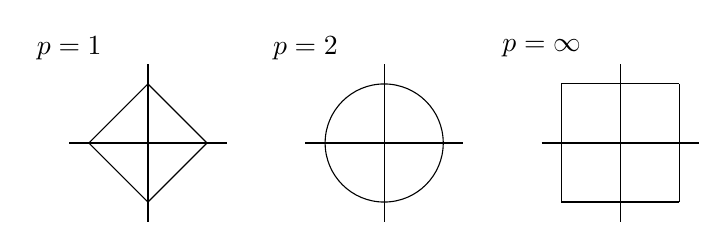
\begin{tikzpicture}
    \draw (-4,0) -- (-2,0); \draw (-3,1) -- (-3,-1); %axes
    % p = 1
    \draw (-3.75, 0) -- (-3, .75); \draw (-3, .75) -- (-2.25, 0); \draw (-2.25,0) -- (-3,-.75); \draw (-3,-.75) -- (-3.75, 0);
    \draw (-4,1.2) node {$p = 1$};
    
    \draw (-1,0) -- (1,0); \draw (0,1) -- (0,-1); %axes
    % p = 2
    \draw (0,0) circle(.75);
    \draw (-1,1.2) node {$p = 2$};
    
    \draw (2,0) -- (4,0); \draw (3,1) -- (3,-1); %axes
    % p = infinity
    \draw (2.25,.75) -- (3.75,.75); \draw (3.75, .75) -- (3.75, -.75); \draw (3.75, -.75) -- (2.25, -.75); \draw (2.25, -.75) -- (2.25, .75);
    \draw (2,1.2) node {$p = \infty$};
    
    \end{tikzpicture}
\end{center}

\begin{theorem}[Minkowski's Theorem]
$||f + g||_p \leq ||f||_p + ||g||_p$.
\end{theorem}
\begin{proof}
\textcolor{red}{Proof needed}
\end{proof}

\begin{theorem}[Riesz-Fischer]
$L^p$ is complete for all $p \in [1, \infty]$
\end{theorem}
\begin{proof}
\textcolor{red}{Proof needed}
\end{proof}

\begin{cor}
$||-||_p$ is a seminorm (fails the 0 only for 0 condition). If we mod out by the relation $f \sim g$ if $f = g$ almost surely, then $||-||_p$ is a Banach space (complete normed vector space).
\end{cor}

The following are some other useful properties of $L^p$ space:
\begin{enumerate}
    \item $L^2$ is a Hilbert Space (a real or complex inner product space that is also a complete metric space).
    \item Embeddings: for $1 \leq p < q \leq \infty$ the following hold:
    \begin{itemize}
        \item $L^q \subset L^p$ if and only if $\om$ does not contain sets of finite but arbitrarily large measure (for instance if $\mu$ is a probability measure).
        \item $L^p \subset L^q$ if and only if $\om$ does not contain sets of nonzero but arbitrarily small measure.
        \item If $\om = \{1,2,...,n\}$, then $L^p \cong L^q \cong \R^n$.
    \end{itemize}
    \item Dual Spaces: For $p,q < \infty$ such that $\frac{1}{p} + \frac{1}{q} = 1$, $L^p$ and $L^q$ are dual to each other as Banach spaces, with identification given by $T_g f = \int fg d\mu$. If $\mu$ is $\sigma$-finite, then $(L^1)^* \cong L^{\infty}$ but we only have that $(L^{\infty})^* \subset L^1$.
    \item For $|\om| = n$, if $p > q$, then $||x||_p \leq ||x||_q \leq n^{1/q - 1/p} ||x||_p$ (and thus they induce the same topology).
\end{enumerate}

\begin{prop}
For $r > s \geq 1$, convergence in $L^r$ implies convergence in $L^s$ but not vice versa.
\end{prop}

\begin{prop}
Both almost sure convergence and $L^p$ convergence imply convergence in distribution
\end{prop}

\subsection{Independence}
\begin{definition}[Independent Sets]
Sets $A_1,..., A_n$ are indpendant if for all $I \subset \{1,...,n\}$, 
\[\prob(\bigcap_{i \in I} A_i) = \prod_{i \in I} \prob(A_i)\]
\end{definition}

\begin{definition}[Independent Random Variables]
Real valued random variables $X_1,...,X_n$ are independent if for all $B_1, ..., B_n \in \cB$,
\[\prob(\bigcap_{i=1}^n\{X_i \in B_i\}) = \prod_{i = 1}^n \prob(X_i \in B_i)\]
An infinite sequence of random variables is said to be independent if every finite subset is independent.
\end{definition}

\begin{definition}[Independent $\sigma$-Algebras]
$\sigma$-algebras $\cF_1,...,\cF_n \subset \cF$ are independent if for all $A_1 \in \cF_i, ..., A_n \in \cF_n$,
\[\prob(\bigcap_{i = 1}^n A_i) = \prod_{i = 1}^n \prob(A_i)\]
\end{definition}

\begin{remark}
Random variables $X_1,..., X_n$ independent is equivalent to the $\sigma$-algebras $\sigma(X_1) ... \sigma(X_n)$ independent.
\end{remark}

\begin{remark}
Pairwise independence is not as strong as collective independence. For instance, let $X_1, X_2, X_3$ be i.i.d $Bernoulli(1/2)$ random variables. Then we have that the following sets are pairwise independent, but not collectively independent:
\[A_1 = \{X_2 = X_3\} \quad A_2 = \{X_1 = X_3\} \quad A_3 = \{X_1 = X_2\}\]
each individually has probability $1/2$, and the intersection of any 2 sets is $\{X_1 = X_2 = X_3\}$ which has probability $1/4$, however the intersection of all 3 is still $\{X_1 = X_2 = X_3\}$ which has probability $1/4 \neq (1/2)^3$.
\end{remark}

\begin{theorem}
For random variables $X_1,...,X_n$, to prove independence it is sufficient to check that for all $x_1,...,x_n \in (- \infty, \infty),$
\[\prob(X_1 < x_1,...,X_n < x_n) = \prod \prob(X_i < x_i)\]
\end{theorem}
\begin{proof}
\textcolor{red}{$\pi-\lambda$ system proof in Durrett}
\end{proof}

\begin{prop}
If $(X_1,...,X_n)$ are absolutely continuous random variables (i.e. they have density $f(x_1,...,x_n)$) then $X_1,...,X_n$ are independent if and only if $f(x_1,...,x_n) = g_1(x_1)...g_n(x_n).$
\end{prop}
\begin{proof}
We can write,
\[\prob(X_1 < x_1, ..., X_n < x_n) = \int_{y_i < x_i} f(y_1,...,y_n)d\Vec{y} = \int_{-\infty}^{x_n} ... \int_{-\infty}^{x_1} g_1(y_1)...g_n(y_n) dy_1...dy_n\]
\[ = \prod_{i = 1}^n (\int_{-\infty}^{x_i} g_i(y_i) dy_i) = \prod_{i = 1}^n \prob(X_i < x_i)\]
\end{proof}

The following are additional properties of independence:
\begin{enumerate}
    \item Functions of independent random variables are independent.
    \item If $X, Y$ are independent with distribution $\mu, \nu$ respectively, and $h: \R^2 \to \R$ is such that either $h \geq 0$ or $\E[|h(X,Y)|] < \infty$, then $\E[h(X,Y)] = \int \int h(x,y) d\mu(x) d\nu(y)$.
    \item If $X_1,...,X_n$ are independent random variables with $X_i \sim \mu_i$, then $(X_1,...,X_n) \sim \mu_1 \times ... \mu_n$
\end{enumerate}

Distribution functions for sums of independent random variables can be given by convolutions of their distribution functions. Let $X$ and $Y$ be independent with $X$ having density function $f$ and $Y$ having density function $g$. Then their sum $X + Y$ has density function,
\[h(z) = (f*g)(z) = \int_{-\infty}^{\infty} f(x) g(z-x) dx = \int_{- \infty}^{\infty} g(y) f(z-y) dy\]
\textcolor{red}{PDFs or CDFs?}

\paragraph{Constructions of Infinite Sequences of Independent Random Variables}
\textcolor{red}{Fill in form page 36 of notes, too tired to do it now}

We now can prove a slightly weaker converse to the first Borel-Cantelli Lemma:

\begin{lemma}[Borel-Cantelli Lemma (2)]
    If $A_n$ are independent, then $\sum_{n = 1}^{\infty} \prob(A_n) = \infty$ implies that $\prob(\limsup_{n \to \infty}A_n) = 1$.
\end{lemma}
\begin{proof}
    We assume the inequality $1 - x \leq e^{-x}$ for $x \in [0,1]$. Then we have that,
    \[\prob((\bigcup_{n = m}^N A_n)^c) = \prob(\bigcap_{n = m}^N A_n^c) = \prod_{n = m}^N (1- \prob(A_n)) \leq e^{-\sum_{n = m}^N \prob(A_n)} \xrightarrow{N \to \infty} 0\]
    Which then implies that $\lim_{N \to \infty} \prob(\bigcup_{n = m}^N A_n) = 1$ for all $m$.
\end{proof}



\subsection{Laws of Large Numbers}
\subsubsection{$L^2$ Law of Large Numbers}
\begin{definition}
    2 random variables $X,Y$ are uncorrelated if $\E[XY] = \E[X]\E[Y]$ or equivalently if,
    \[Cov(X,Y) = \E[(X -\E[X])(Y - \E[Y])] = 0\]
\end{definition}
\begin{remark}
    This is weaker than independence.
\end{remark}

\begin{theorem}[$L^2$ Law of Large Numbers]
    Let $X_1,...,X_n \in L^2(\om)$ be uncorrolated random variables. Then $Var(X_1+ ... + X_n) = Var(X_1)+...+ Var(X_n)$.
\end{theorem}
\begin{proof}
    \textcolor{red}{Proof}
\end{proof}

\begin{remark}
    Note that this implies that if $X_1, X_2,...$ are $i.i.d.$ with variance $Var(X_i) = \sigma^2$, then we have that,
    \[\lim_{n \to \infty} Var(\frac{X_1 + ... + X_n}{n}) = \lim_{n \to \infty} \frac{1}{n^2} Var(X_1 + ... + X_n) = \lim_{n \to \infty} \frac{\sigma^2}{n} = 0\]
    Then we have that $\frac{\sum_{i = 1}^n X_i}{n}$ converges to a constant in $L^2$. Furthermore, convergence in $L^2$ implies convergence in $L^1$, thus $X_n \to \mu$ for $\mu = \E[X_i].$
\end{remark}

\subsubsection{Weak Law of Large Numbers}
\begin{theorem}[Weak Law of Large Numbers]
    Let $X_1, X_2, ...$ be i.i.d. with $\E[|X_i|] < \infty$, and set $S_n = X_1 + ... + X_n$, $\mu = \E[X_i]$. Then as $n \nearrow \infty$, 
    \[\frac{S_n}{n} \xlongrightarrow{p} \mu\]
\end{theorem}
\begin{proof}
    We begin by truncating our random variables $X_i$ by a cutoff $c > 0$. Let $X_i^c = X_i 1_{|X_i| < c}$, and define $Y_i^c = X_i - X_i^c$. Then we have,
    \[\frac{1}{n} \sum_{i = 1}^n X_i = \frac{1}{n} \sum_{i = 1}^n (X_i^c + Y_i^c) = \frac{1}{n} \sum_{i = 1}^n X_i^c + \frac{1}{n} \sum_{i = 1}^n Y_i^c\]
    Let $\xi_n^c = \frac{1}{n} \sum_{i = 1}^n X_i^c$ and $\eta_n^c = \frac{1}{n} \sum_{i = 1}^n Y_i^c$, and define, $a_c = \E[X_i^c], b_c = \E[Y_i^c]$. Then we have,
    \[\delta_n = \E[|\frac{S_n}{n} - \mu|] = \E[|\xi_n^c + \eta_n^c - \mu|] \leq \E[|\xi_n^c - a_c|] + \E[|\eta_n^c - b_c|] \leq \E[|\xi_n^c - a_c|] + 2\E[|Y_i^c|]\]
    Now note that $X_i^c$ is bounded and therefore has finite second moment. Thus, we can apply the $L^2$ law of large numbers and see that $\xi_n^c \xrightarrow{p} a_c$, so we get,
    \[\limsup_{n \to \infty} \delta_n \leq 2\E[|Y_i^c|]\]
    $Y_i^c \xrightarrow{a.s.} 0$, so we can apply dominated convergence theorem with $X_i$ as the bounding variable to see that $2\E[|Y_i^c|] \xrightarrow{c \to \infty} 0$, concluding the proof.

    \textcolor{red}{In my notes I have at the end the phrase "slightly different version with slightly different hypothesis." What is that referring to? Applying the statement of the $L^2$ law of large numbers?}
\end{proof}


\subsubsection{Strong Law of Large Numbers}
We now move onto the strong laws of large numbers, considered strong because they prove almost sure convergence rather than convergence in probability (or $L^2$).
\begin{theorem}[$L^4$ Strong Law of Large Numbers]
    Let $X_i$ be i.i.d. random variables with $\E[X_i] = \mu$ and $\E[X_i^4] < \infty$, then $S_n = X_1 + ... + X_n$, $\frac{S_n}{n} \to \mu$ a.s.
\end{theorem}
\begin{proof}
    We can assume $\mu = 0$ by replacing $X_i$ with $X_i - \mu$. Then we have,
    \[\E[S_n^4] = \sum_{i = 1}^n \E[X_i^4] + \binom{4}{2} \sum_{1 \leq i<j \leq n} \E[X_i^2]\E[X_j^2] = n\E[X_i^4] + 3n(n-1)\E[X_i^2] \leq cn^2\]
    Then we have that 
    \[
        \prob(|S_n| > n \vep) \leq \frac{\E[S_n^4]}{(n\vep)^4} \leq \frac{cn^2}{(n\vep)^4} \leq \frac{1}{n^2 \vep^4}
    \]
    So we have by Borel-Cantelli, $\prob(|S_n| > n \vep \text{ infinitely often}) = 0$
\end{proof}


\begin{theorem}[Strong Law of Large Numbers]
    Let $X_1,X_2,...$ be pairwise independent identically distributed random variables with $\E[|X_i|] < \infty$, $\E[X_i] = \mu$. Then,
     \[ \frac{S_n}{n} \xrightarrow{a.s.} \mu\]
    Additionally, if $\E[X_i^+] = \infty$ and $\E[X_i^-] < \infty$, then $\frac{S_n}{n} \to \infty$ almost surely.
\end{theorem}
We will give two proofs of the strong law of large numbers, the first of which is due to Etemadi in 1981:
\begin{proof}
    \textcolor{red}{need proof of the second statement, should be an application of Borel-Cantelli?}
    Just as in the proof of the weak law of large numbers, we begin by truncating. Let $Y_k = X_k 1_{|X_k|\leq k}$. We first show that it is sufficient to prove the convergence of the truncated variables.
    \begin{lemma}
        Let $T_n = Y_1 + ... + Y_n$. It is sufficient to show that $\frac{T_n}{n} \xrightarrow{a.s.} \mu$.
    \end{lemma}
    \begin{proof}
        $\sum_{k = 1}^{\infty} \prob(|X_k| > k) \leq \int_0^{\infty} \prob(|X_1| > t) dt = \E[|X_i|] < \infty$ so by Borel-Cantelli we have that $\prob(X_k \neq Y_k \text{ infinitely often}) = 0$ Therefore we have that for every $\omega \in \om$ except on a measure $0$ set, there exists a $R(\omega) < \infty$ such that $|S_n(\omega) - T_n(\omega)| < R(\omega)$, so $|\frac{S_n(\omega)}{n} - \frac{T_n(\omega)}{n}| < \frac{R(\omega)}{n} \xrightarrow{n \to \infty} 0.$
    \end{proof}
    \begin{lemma}
        $\sum_{k = 0}^{\infty} \frac{Var(Y_k)}{k^2} \leq 4 \E[X_1] < \infty$
    \end{lemma}
    \begin{proof}
        $Var(Y_k) \leq \E[Y_k^2] = \int_0^{\infty} 2y \prob(|Y_k| > y)dy $\textcolor{red}{why?}$ \leq \int_0^k 2y \prob(|X_1| > y)$ \textcolor{red}{why not equal?}

        Since everything is $\geq 0$, we can apply Fubini's theorem to see,
        \[\sum_{k = 1}^{\infty} \frac{\E[Y_k^2]}{k^2} \leq \sum_{k = 1}^{\infty} 
        \frac{1}{k^2} \int_0^{\infty} 1_{y < k} 2y \prob(|X_1| > k) dy = \int_0^{\infty} (\sum_{k = 1}^{\infty} \frac{1_{y < k}}{k^2}) 2y\prob(|X_1|>y)dy\]
        So to complete the proof we show that if $y \geq 0$, then $2y\sum_{k > y} \frac{1}{k^2} \leq 4$. (For this see Lemma 2.4.4 of Durrett, it is not hard).
    \end{proof}
    Now our goal is to combine these two lemmas to prove the Strong Law of Large Numbers.

    The remainder of this proof follows the following outline:
    \begin{enumerate}
        \item Note that we can write $X_n = X_n^+ - X_n^-$, so we can assume that we are working with $X_i>0$ and combine the results for $X^+$ and $X^-$ to obtain the general case.
        \item Choose a subsequence $T_{k_n}$ and show convergence.
        \item Use the monotonicity to conclude that $T_n$ converges almost surely.
    \end{enumerate}

    To choose the subsequence, For some $\alpha > 1$, define $k_n = [\alpha^n]$ (where $[x]$ is defined to be the closest integer to $x$). Then we have that $k_n$ grows exponentially. So now we have,
    \[\sum_{n = 1}^{\infty} \prob(|T_{k_n} - \E[T_{k_n}]| > \vep k_n) \leq \frac{1}{\vep^2} \sum_{n = 1}^{\infty} \frac{Var(T_{k_n})}{k_n^2} = \frac{1}{\vep^2} \sum_{n=1}^{\infty} \frac{1}{k_n^2} \sum_{m = 1}^{k_n} Var(Y_m) \]
    \[= \frac{1}{\vep^2} \sum_{m = 1}^{\infty} Var(Y_m) \sum_{k_n \geq m} \frac{1}{k_n^2} \leq 4(1-\frac{1}{\alpha^2})^{-1}\frac{1}{\vep^2}\sum_{m = 1}^{\infty} \frac{\E[Y_m^2]}{m^2} < \infty\]
    Thus by Borel-Cantelli we can conlude that,
    \[ \frac{T_{n_k} - \E[T_{n_k}]}{n_k} \xrightarrow{a.s.} 0\]
    Note that this is sufficient to show this subsequence converges to $\mu$ as this implies that,
    \[\lim_{k \to \infty} \frac{T_{n_k}}{n_k} = \lim_{k \to \infty} \frac{\E[T_{n_k}]}{n_k} = \lim_{k \to \infty} \frac{\E[S_{n_k}]}{n_k}  = \mu\]

    Now to handle the intermediate values we have the following inequality for $k_n \leq m \leq k_{n+1}$:
    \[\frac{T_{k_n}}{k_{n+1}} \leq \frac{T_m}{m} \leq \frac{T_{k_{n+1}}}{k_n}\]
    So then this implies that,
    \[(\frac{k_{n}}{k_{n+1}})\frac{T_{n_k}}{n_k} \leq \frac{T_m}{m} \leq (\frac{k_{n+1}}{k_n})\frac{T_{k_{n+1}}}{n_{k+1}}\]
    and by our choice of subsequence we have that $\frac{k_{n+1}}{k_n} \to \alpha$ as $n \to \infty$, for arbitrarily chosen $\alpha > 1$, thus,
    \[\mu \leq \liminf_{m \to \infty} \frac{T_m}{m} \leq \limsup_{m \to \infty} \frac{T_m}{m} \leq \mu\]
    which concludes the first proof.
\end{proof}

To present the second proof we first need to prove the following theorems of Kolmogorov:

\begin{theorem}[Kolmogorov's Maximal Inequality]
    Let $X_1, X_2,...$ be independent centered random variables with $Var(X_i) < \infty$. Let $S_n = X_1 + ... + X_n$. Then,
    \[
        \prob(\max_{1 \leq k \leq n} |S_k| \geq x) \leq \frac{Var(S_n)}{x^2}
    \] 
\end{theorem}
\begin{remark}
    Note that this is stronger than the Chebyshev inequality since we take the maximum over all $S_k$ for $k \leq n$.
\end{remark}
\begin{proof}
    Define $A_k = \{|S_k| \geq x, |S_j| < x \text{ for all } j < k\}$. Note that the $A_k$ are disjoint, and that $\bigcup_{k = 1}^n A_k = \{\max_{1 \leq k \leq n} |S_k| \geq x\}$. Then we have,
    \[\E[S+n^2] = \sum_{k =1}^n \int_{A_k} S_n^2 d \prob ... \]
    \textcolor{red}{UNFINISHED IN MY NOTES see Durrett to finish}
\end{proof}

\begin{theorem}[Kolmogorov 0-1 Law]
    Define $\cF_n' = \sigma(X_n, X_{n+1},...)$ the smallest $\sigma$-field such that all $X_m, m \geq n$ are measurable. Define the tail $\sigma$-field $\mathcal{T}= \bigcap_{n = 1}^{\infty}$. If the sequence $X_1, X_2, ...$ are independent, then for an $A \in \mathcal{T}$, $\prob(A) = 0$ or $1$.
\end{theorem}

\begin{proof}
    The idea of the proof is to show that $A$ is independent from itself and therefore must have probability either 0 or 1. This requires $\pi = \lambda$ systems and can be found in Durrett \textcolor{red}{REVISIT IF YOU EVER GET AROUND TO $\pi-\lambda$ STUFF}
\end{proof}

We use these two theorems to prove the following theorem that we will the apply to give a second proof of the Strong Law of Large Numbers.

\begin{theorem}[Kolmogorov's One Series Theorem]
    Suppose $X_1, X_2,...$ are independent centered random variables. If $\sum_{i = 0}^{\infty} Var(X_i) < \infty$, then with probability 1,
    \[\sum_{i = 1}^{\infty} X_i(\omega)\]
    converges.
\end{theorem}
\begin{proof}
    Let $S_n$ be the $n$-th partial sum of the series. To prove this we will prove
    $$\prob(\{S_n\}_n \text{ is Cauchy})= 1$$
    By Kolmogorov's maximal inequality we have,
    \[\prob(\max_{M \leq m \leq N}|S_m - S_M| > \vep) \leq \frac{1}{\vep^2} Var(S_N- S_M) = \frac{1}{\vep^2} \sum_{n = M+1}^N Var(X_n) < \infty\]
    So we have,
    \[\prob(\sup_{m,n \geq M} |S_m - S_n| > 2\vep) \leq \prob(\sup_{m \geq M} |S_m - S_M| > \vep) \xrightarrow{M \to \infty} 0\]
\end{proof}

We also will need the following lemma, which we won't prove here,

\begin{lemma}[Kronecker's Lemma]
    If $a_n \to \infty$ and $\{x_n\}_n$ is such that $\sum_{i = 1}^{\infty} \frac{x_n}{a_n}$ converges then $\frac{1}{a_n} \sum_{i = 1}^n x_n \xrightarrow{n \to \infty} 0$.
\end{lemma}

Now we give the second proof of the Strong Law of Large Numbers:
\begin{proof}
    Again, let $Y_k = X_k1_{|X_k| \leq k}$, and let $Z_k = Y_k - \E[Y_k]$. Recall that by lemma 4 of proof 1 it is sufficient to show to show that $\frac{T_n - \E[T_n]}{n} \to 0$ almost surely. We have, $Var(\frac{Z_k}{k}) = \frac{Var(Y_k)}{k^2} < \infty$ by lemma 5 in the first proof, therefore by Kolmogorov's one series theorem, $\sum_{k = 1}^{\infty} \frac{Z_k}{k}$ converges almost surely. By Kronecker's lemma, this implies that $\frac{1}{n} \sum_{k = 1}^n Z_k \to 0$ almost surely, so, 
    \[\frac{1}{n} \sum_{k = 1}^n Z_k = \frac{\sum_{k = 1}^nY_k - \E[Y_k]}{n}= \frac{T_n - \E[T_n]}{n} \xrightarrow{a.s.} 0\]
\end{proof}

\subsubsection{Applications}
The following are examples of applications of the laws of large numbers chosen from Durrett,

\paragraph{Bernstein Polynomials}
Let $f$ be continuous on $[0,1]$, and define the \textit{$n$-th Bernstein polynomial of $f$} to be,
\[ f_n(x) = \sum_{m = 0}^n \binom{n}{m} x^m(1-x)^{n-m} f(\frac{m}{n}) \]
Then $\sup_{x \in I}|f_n(x) - f(x)| \xrightarrow{n \to \infty} 0$.

\begin{proof}
    Let $X_i \sim Bern(p)$, $S_n = X_1 + ... + X_n$, then we have that, $\prob(S_n = m) = \binom{n}{m} p^m(1-p)^{n-m}$. Therefore,
    \[f_n(p) = \E[f(\frac{S_n}{n})] \xrightarrow{n \to \infty} f(p)\]
\end{proof}


\paragraph{High-Dimensional Cubes Concentrate on the Boundary of a Ball} 
Let $X_i \sim Unif[-1,1]$, $Y_i = X_i^2$, Then we can easilyt see that $\E[Y_i] = \frac{1}{3}$ and $Var(Y_i) \leq 1$. Thus by the law of large numbers we have,
\[\frac{X_1^2+...+X_n^2}{n} \xrightarrow{n \to \infty} \frac{1}{3}\]
Therefore, by the law of large numbers, for some small $\delta > 0$, the $\delta$-neighborhood of the ball $B(0, \sqrt{\frac{n}{3}})$ contains almost all of the mass of the cube.

\begin{comment}
\paragraph{Record Values}
Let $X_1, X_2, ... $ be i.i.d. random variables distributed according to some continuous distribution. Let $A_k$ be the event that $X_k$ sets a record, that is, $A_k = \{X_k > \sup_{j \leq k} X_j\}$. Perhaps unintuitively, the $A_k$ are independent events, and $\prob(A_k) = \frac{1}{k}$

\begin{proof}
    For every $n$ we can define the random variable $\pi \in S_n$ such that $\pi(\omega)$ is such that $X_{\pi(\omega)(1)} \leq ... \leq X_{\pi(\omega)(n)}$. By the $i.i.d.$ property of the $X_i$'s, $\pi$ is uniform on $S_n$, so $\prob(A_n) = \prob(\pi(n) = n) = \frac{1}{n}$
\end{proof}
\end{comment}

\paragraph{Renewal Theorem} Let $X_1, X_2, ... $ be i.i.d. random bariables with $0 < X_i < \infty$. Define $T_n = X_1 + ... + X_n$ and let $\E[X_i] = \mu$. Define $N_t = \sup\{n| T_n \leq t\}$ By the law of large numbers we have that $\frac{S_n}{n} \xrightarrow{a.s.} \mu$, and we claim that $\frac{N_t}{t} \xrightarrow{a.s.} \frac{1}{\mu}$.
\begin{proof}
    $T_{N_t} \leq t \leq T_{N_t + 1}$, so
    \[\frac{T_{N_t}}{N_t} \leq \frac{t}{N_t} \leq \frac{T_{N_t + 1}}{N_t+1} (\frac{N_t + 1}{N_t})\]
    Both the right hand side and left hand side go to $\mu$ as $t \to \infty$ by the law of large numbers so we are done.
\end{proof}


\paragraph{Triangular Arrays}


\subsection{Central Limit Theorem}
\subsubsection{Characteristic Functions}






\subsection{Markov Chains}


\subsection{Martingales}
\subsubsection{Radon-Nikodym Theorem}

\begin{definition}[Absolute Continuity]
\textcolor{red}{Definition}
\end{definition}



\begin{definition}[Radon-Nikodym Derivative]
\end{definition}


\begin{theorem}[Radon-Nikodym Theorem]
    
\end{theorem}



\subsection{Large Deviation Principles}

\subsection{Stein's Method}